\documentclass[1p]{elsarticle_modified}
%\bibliographystyle{elsarticle-num}

%\usepackage[colorlinks]{hyperref}
%\usepackage{abbrmath_seonhwa} %\Abb, \Ascr, \Acal ,\Abf, \Afrak
\usepackage{amsfonts}
\usepackage{amssymb}
\usepackage{amsmath}
\usepackage{amsthm}
\usepackage{scalefnt}
\usepackage{amsbsy}
\usepackage{kotex}
\usepackage{caption}
\usepackage{subfig}
\usepackage{color}
\usepackage{graphicx}
\usepackage{xcolor} %% white, black, red, green, blue, cyan, magenta, yellow
\usepackage{float}
\usepackage{setspace}
\usepackage{hyperref}

\usepackage{tikz}
\usetikzlibrary{arrows}

\usepackage{multirow}
\usepackage{array} % fixed length table
\usepackage{hhline}

%%%%%%%%%%%%%%%%%%%%%
\makeatletter
\renewcommand*\env@matrix[1][\arraystretch]{%
	\edef\arraystretch{#1}%
	\hskip -\arraycolsep
	\let\@ifnextchar\new@ifnextchar
	\array{*\c@MaxMatrixCols c}}
\makeatother %https://tex.stackexchange.com/questions/14071/how-can-i-increase-the-line-spacing-in-a-matrix
%%%%%%%%%%%%%%%

\usepackage[normalem]{ulem}

\newcommand{\msout}[1]{\ifmmode\text{\sout{\ensuremath{#1}}}\else\sout{#1}\fi}
%SOURCE: \msout is \stkout macro in https://tex.stackexchange.com/questions/20609/strikeout-in-math-mode

\newcommand{\cancel}[1]{
	\ifmmode
	{\color{red}\msout{#1}}
	\else
	{\color{red}\sout{#1}}
	\fi
}

\newcommand{\add}[1]{
	{\color{blue}\uwave{#1}}
}

\newcommand{\replace}[2]{
	\ifmmode
	{\color{red}\msout{#1}}{\color{blue}\uwave{#2}}
	\else
	{\color{red}\sout{#1}}{\color{blue}\uwave{#2}}
	\fi
}

\newcommand{\Sol}{\mathcal{S}} %segment
\newcommand{\D}{D} %diagram
\newcommand{\A}{\mathcal{A}} %arc


%%%%%%%%%%%%%%%%%%%%%%%%%%%%%5 test

\def\sl{\operatorname{\textup{SL}}(2,\Cbb)}
\def\psl{\operatorname{\textup{PSL}}(2,\Cbb)}
\def\quan{\mkern 1mu \triangleright \mkern 1mu}

\theoremstyle{definition}
\newtheorem{thm}{Theorem}[section]
\newtheorem{prop}[thm]{Proposition}
\newtheorem{lem}[thm]{Lemma}
\newtheorem{ques}[thm]{Question}
\newtheorem{cor}[thm]{Corollary}
\newtheorem{defn}[thm]{Definition}
\newtheorem{exam}[thm]{Example}
\newtheorem{rmk}[thm]{Remark}
\newtheorem{alg}[thm]{Algorithm}

\newcommand{\I}{\sqrt{-1}}
\begin{document}

%\begin{frontmatter}
%
%\title{Boundary parabolic representations of knots up to 8 crossings}
%
%%% Group authors per affiliation:
%\author{Yunhi Cho} 
%\address{Department of Mathematics, University of Seoul, Seoul, Korea}
%\ead{yhcho@uos.ac.kr}
%
%
%\author{Seonhwa Kim} %\fnref{s_kim}}
%\address{Center for Geometry and Physics, Institute for Basic Science, Pohang, 37673, Korea}
%\ead{ryeona17@ibs.re.kr}
%
%\author{Hyuk Kim}
%\address{Department of Mathematical Sciences, Seoul National University, Seoul 08826, Korea}
%\ead{hyukkim@snu.ac.kr}
%
%\author{Seokbeom Yoon}
%\address{Department of Mathematical Sciences, Seoul National University, Seoul, 08826,  Korea}
%\ead{sbyoon15@snu.ac.kr}
%
%\begin{abstract}
%We find all boundary parabolic representation of knots up to 8 crossings.
%
%\end{abstract}
%\begin{keyword}
%    \MSC[2010] 57M25 
%\end{keyword}
%
%\end{frontmatter}

%\linenumbers
%\tableofcontents
%
\newcommand\colored[1]{\textcolor{white}{\rule[-0.35ex]{0.8em}{1.4ex}}\kern-0.8em\color{red} #1}%
%\newcommand\colored[1]{\textcolor{white}{ #1}\kern-2.17ex	\textcolor{white}{ #1}\kern-1.81ex	\textcolor{white}{ #1}\kern-2.15ex\color{red}#1	}

{\Large $\underline{12n_{0799}~(K12n_{0799})}$}

\setlength{\tabcolsep}{10pt}
\renewcommand{\arraystretch}{1.6}
\vspace{1cm}\begin{tabular}{m{100pt}>{\centering\arraybackslash}m{274pt}}
\multirow{5}{120pt}{
	\centering
	\includegraphics[width=112pt]{../../../GIT/diagram.site/Diagrams/png/2888_12n_0799.png}\\
\ \ \ A knot diagram\footnotemark}&
\allowdisplaybreaks
\textbf{Linearized knot diagam} \\
\cline{2-2}
 &
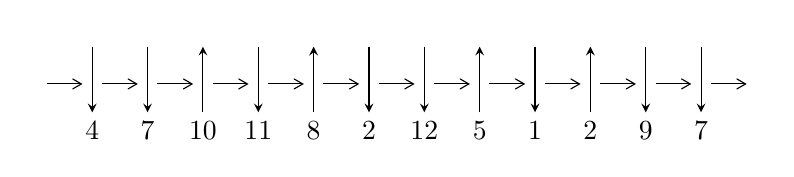
\begin{tikzpicture}[x=20pt, y=17pt]
	% nodes
	\node (C0) at (0, 0) {};
	\node (C1) at (1, 0) {};
	\node (C1U) at (1, +1) {};
	\node (C1D) at (1, -1) {4};

	\node (C2) at (2, 0) {};
	\node (C2U) at (2, +1) {};
	\node (C2D) at (2, -1) {7};

	\node (C3) at (3, 0) {};
	\node (C3U) at (3, +1) {};
	\node (C3D) at (3, -1) {10};

	\node (C4) at (4, 0) {};
	\node (C4U) at (4, +1) {};
	\node (C4D) at (4, -1) {11};

	\node (C5) at (5, 0) {};
	\node (C5U) at (5, +1) {};
	\node (C5D) at (5, -1) {8};

	\node (C6) at (6, 0) {};
	\node (C6U) at (6, +1) {};
	\node (C6D) at (6, -1) {2};

	\node (C7) at (7, 0) {};
	\node (C7U) at (7, +1) {};
	\node (C7D) at (7, -1) {12};

	\node (C8) at (8, 0) {};
	\node (C8U) at (8, +1) {};
	\node (C8D) at (8, -1) {5};

	\node (C9) at (9, 0) {};
	\node (C9U) at (9, +1) {};
	\node (C9D) at (9, -1) {1};

	\node (C10) at (10, 0) {};
	\node (C10U) at (10, +1) {};
	\node (C10D) at (10, -1) {2};

	\node (C11) at (11, 0) {};
	\node (C11U) at (11, +1) {};
	\node (C11D) at (11, -1) {9};

	\node (C12) at (12, 0) {};
	\node (C12U) at (12, +1) {};
	\node (C12D) at (12, -1) {7};
	\node (C13) at (13, 0) {};

	% arrows
	\draw[->,>={angle 60}]
	(C0) edge (C1) (C1) edge (C2) (C2) edge (C3) (C3) edge (C4) (C4) edge (C5) (C5) edge (C6) (C6) edge (C7) (C7) edge (C8) (C8) edge (C9) (C9) edge (C10) (C10) edge (C11) (C11) edge (C12) (C12) edge (C13) ;	\draw[->,>=stealth]
	(C1U) edge (C1D) (C2U) edge (C2D) (C3D) edge (C3U) (C4U) edge (C4D) (C5D) edge (C5U) (C6U) edge (C6D) (C7U) edge (C7D) (C8D) edge (C8U) (C9U) edge (C9D) (C10D) edge (C10U) (C11U) edge (C11D) (C12U) edge (C12D) ;
	\end{tikzpicture} \\
\hhline{~~} \\& 
\textbf{Solving Sequence} \\ \cline{2-2} 
 &
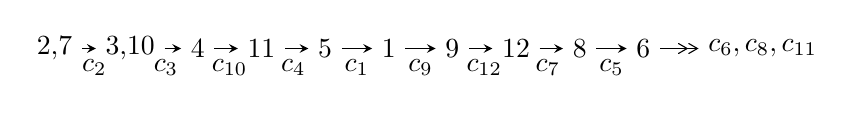
\begin{tikzpicture}[x=23pt, y=7pt]
	% node
	\node (A0) at (-1/8, 0) {2,7};
	\node (A1) at (17/16, 0) {3,10};
	\node (A2) at (17/8, 0) {4};
	\node (A3) at (25/8, 0) {11};
	\node (A4) at (33/8, 0) {5};
	\node (A5) at (41/8, 0) {1};
	\node (A6) at (49/8, 0) {9};
	\node (A7) at (57/8, 0) {12};
	\node (A8) at (65/8, 0) {8};
	\node (A9) at (73/8, 0) {6};
	\node (C1) at (1/2, -1) {$c_{2}$};
	\node (C2) at (13/8, -1) {$c_{3}$};
	\node (C3) at (21/8, -1) {$c_{10}$};
	\node (C4) at (29/8, -1) {$c_{4}$};
	\node (C5) at (37/8, -1) {$c_{1}$};
	\node (C6) at (45/8, -1) {$c_{9}$};
	\node (C7) at (53/8, -1) {$c_{12}$};
	\node (C8) at (61/8, -1) {$c_{7}$};
	\node (C9) at (69/8, -1) {$c_{5}$};
	\node (A10) at (11, 0) {$c_{6},c_{8},c_{11}$};

	% edge
	\draw[->,>=stealth]	
	(A0) edge (A1) (A1) edge (A2) (A2) edge (A3) (A3) edge (A4) (A4) edge (A5) (A5) edge (A6) (A6) edge (A7) (A7) edge (A8) (A8) edge (A9) ;
	\draw[->>,>={angle 60}]	
	(A9) edge (A10);
\end{tikzpicture} \\ 

\end{tabular} \\

\footnotetext{
The image of knot diagram is generated by the software ``\textbf{Draw programme}" developed by Andrew Bartholomew(\url{http://www.layer8.co.uk/maths/draw/index.htm\#Running-draw}), where we modified some parts for our purpose(\url{https://github.com/CATsTAILs/LinksPainter}).
}\phantom \\ \newline 
\centering \textbf{Ideals for irreducible components\footnotemark of $X_{\text{par}}$} 
 
\begin{align*}
I^u_{1}&=\langle 
5.00355\times10^{780} u^{109}+4.44505\times10^{780} u^{108}+\cdots+9.26593\times10^{783} b+8.56922\times10^{784},\\
\phantom{I^u_{1}}&\phantom{= \langle  }4.02128\times10^{784} u^{109}+2.31943\times10^{784} u^{108}+\cdots+2.42490\times10^{787} a-8.43979\times10^{788},\\
\phantom{I^u_{1}}&\phantom{= \langle  }u^{110}+u^{109}+\cdots+73536 u+2617\rangle \\
I^u_{2}&=\langle 
2.23748\times10^{66} u^{40}-3.11786\times10^{66} u^{39}+\cdots+5.39174\times10^{65} b-5.51085\times10^{66},\\
\phantom{I^u_{2}}&\phantom{= \langle  }1.57158\times10^{65} u^{40}-2.36554\times10^{65} u^{39}+\cdots+8.04737\times10^{63} a-3.17576\times10^{65},\;u^{41}- u^{40}+\cdots-3 u-1\rangle \\
I^u_{3}&=\langle 
b+u-1,\;a+u,\;u^2- u+1\rangle \\
\\
\end{align*}
\raggedright * 3 irreducible components of $\dim_{\mathbb{C}}=0$, with total 153 representations.\\
\footnotetext{All coefficients of polynomials are rational numbers. But the coefficients are sometimes approximated in decimal forms when there is not enough margin.}
\newpage
\renewcommand{\arraystretch}{1}
\centering \section*{I. $I^u_{1}= \langle 5.00\times10^{780} u^{109}+4.45\times10^{780} u^{108}+\cdots+9.27\times10^{783} b+8.57\times10^{784},\;4.02\times10^{784} u^{109}+2.32\times10^{784} u^{108}+\cdots+2.42\times10^{787} a-8.44\times10^{788},\;u^{110}+u^{109}+\cdots+73536 u+2617 \rangle$}
\flushleft \textbf{(i) Arc colorings}\\
\begin{tabular}{m{7pt} m{180pt} m{7pt} m{180pt} }
\flushright $a_{2}=$&$\begin{pmatrix}1\\0\end{pmatrix}$ \\
\flushright $a_{7}=$&$\begin{pmatrix}0\\u\end{pmatrix}$ \\
\flushright $a_{3}=$&$\begin{pmatrix}1\\u^2\end{pmatrix}$ \\
\flushright $a_{10}=$&$\begin{pmatrix}-0.00165833 u^{109}-0.000956508 u^{108}+\cdots+262.589 u+34.8048\\-0.000539994 u^{109}-0.000479720 u^{108}+\cdots-211.157 u-9.24809\end{pmatrix}$ \\
\flushright $a_{4}=$&$\begin{pmatrix}0.00355770 u^{109}+0.00302258 u^{108}+\cdots+1068.05 u+35.8465\\-0.0000360471 u^{109}-0.0000574092 u^{108}+\cdots-32.5756 u-1.98675\end{pmatrix}$ \\
\flushright $a_{11}=$&$\begin{pmatrix}-0.00219832 u^{109}-0.00143623 u^{108}+\cdots+51.4314 u+25.5567\\-0.000539994 u^{109}-0.000479720 u^{108}+\cdots-211.157 u-9.24809\end{pmatrix}$ \\
\flushright $a_{5}=$&$\begin{pmatrix}-0.00184498 u^{109}-0.00143087 u^{108}+\cdots-165.261 u+12.2558\\0.0000480912 u^{109}+0.0000500660 u^{108}+\cdots-1.21923 u+0.337163\end{pmatrix}$ \\
\flushright $a_{1}=$&$\begin{pmatrix}0.00130209 u^{109}+0.00107878 u^{108}+\cdots+138.910 u-3.01710\\-0.000105047 u^{109}-0.0000969873 u^{108}+\cdots-24.1334 u-1.41572\end{pmatrix}$ \\
\flushright $a_{9}=$&$\begin{pmatrix}-0.00550803 u^{109}-0.00459500 u^{108}+\cdots-1781.60 u-71.4609\\-0.000407303 u^{109}-0.000383400 u^{108}+\cdots-186.765 u-8.60675\end{pmatrix}$ \\
\flushright $a_{12}=$&$\begin{pmatrix}0.00130209 u^{109}+0.00107878 u^{108}+\cdots+138.910 u-3.01710\\-0.000125326 u^{109}-0.000111403 u^{108}+\cdots-37.1469 u-2.00012\end{pmatrix}$ \\
\flushright $a_{8}=$&$\begin{pmatrix}0.00422116 u^{109}+0.00367787 u^{108}+\cdots+2016.89 u+100.317\\0.0000745344 u^{109}+0.0000765968 u^{108}+\cdots+24.9481 u+1.13426\end{pmatrix}$ \\
\flushright $a_{6}=$&$\begin{pmatrix}- u\\- u\end{pmatrix}$\\&\end{tabular}
\flushleft \textbf{(ii) Obstruction class $= -1$}\\~\\
\flushleft \textbf{(iii) Cusp Shapes $= -0.00328476 u^{109}-0.00285610 u^{108}+\cdots-1147.32 u-43.1143$}\\~\\
\newpage\renewcommand{\arraystretch}{1}
\flushleft \textbf{(iv) u-Polynomials at the component}\newline \\
\begin{tabular}{m{50pt}|m{274pt}}
Crossings & \hspace{64pt}u-Polynomials at each crossing \\
\hline $$\begin{aligned}c_{1}\end{aligned}$$&$\begin{aligned}
&u^{110}-6 u^{109}+\cdots+11 u-2
\end{aligned}$\\
\hline $$\begin{aligned}c_{2},c_{6}\end{aligned}$$&$\begin{aligned}
&u^{110}+u^{109}+\cdots+73536 u+2617
\end{aligned}$\\
\hline $$\begin{aligned}c_{3}\end{aligned}$$&$\begin{aligned}
&u^{110}-14 u^{108}+\cdots+129540868 u+14647477
\end{aligned}$\\
\hline $$\begin{aligned}c_{4}\end{aligned}$$&$\begin{aligned}
&u^{110}-2 u^{109}+\cdots+124018 u-36863
\end{aligned}$\\
\hline $$\begin{aligned}c_{5},c_{8}\end{aligned}$$&$\begin{aligned}
&u^{110}+4 u^{109}+\cdots+45870 u+9829
\end{aligned}$\\
\hline $$\begin{aligned}c_{7},c_{12}\end{aligned}$$&$\begin{aligned}
&u^{110}+2 u^{109}+\cdots-559427 u-79997
\end{aligned}$\\
\hline $$\begin{aligned}c_{9}\end{aligned}$$&$\begin{aligned}
&u^{110}- u^{109}+\cdots+1686688 u-214604
\end{aligned}$\\
\hline $$\begin{aligned}c_{10}\end{aligned}$$&$\begin{aligned}
&u^{110}-7 u^{109}+\cdots+20930122 u+5719333
\end{aligned}$\\
\hline $$\begin{aligned}c_{11}\end{aligned}$$&$\begin{aligned}
&u^{110}+10 u^{109}+\cdots-1755 u-172
\end{aligned}$\\
\hline
\end{tabular}\\~\\
\newpage\renewcommand{\arraystretch}{1}
\flushleft \textbf{(v) Riley Polynomials at the component}\newline \\
\begin{tabular}{m{50pt}|m{274pt}}
Crossings & \hspace{64pt}Riley Polynomials at each crossing \\
\hline $$\begin{aligned}c_{1}\end{aligned}$$&$\begin{aligned}
&y^{110}-26 y^{109}+\cdots+279 y+4
\end{aligned}$\\
\hline $$\begin{aligned}c_{2},c_{6}\end{aligned}$$&$\begin{aligned}
&y^{110}+83 y^{109}+\cdots-338995270 y+6848689
\end{aligned}$\\
\hline $$\begin{aligned}c_{3}\end{aligned}$$&$\begin{aligned}
&y^{110}-28 y^{109}+\cdots-7442649453513616 y+214548582465529
\end{aligned}$\\
\hline $$\begin{aligned}c_{4}\end{aligned}$$&$\begin{aligned}
&y^{110}-24 y^{109}+\cdots-95798204714 y+1358880769
\end{aligned}$\\
\hline $$\begin{aligned}c_{5},c_{8}\end{aligned}$$&$\begin{aligned}
&y^{110}+52 y^{109}+\cdots+4273725646 y+96609241
\end{aligned}$\\
\hline $$\begin{aligned}c_{7},c_{12}\end{aligned}$$&$\begin{aligned}
&y^{110}+102 y^{109}+\cdots+299723255241 y+6399520009
\end{aligned}$\\
\hline $$\begin{aligned}c_{9}\end{aligned}$$&$\begin{aligned}
&y^{110}+41 y^{109}+\cdots-686133223824 y+46054876816
\end{aligned}$\\
\hline $$\begin{aligned}c_{10}\end{aligned}$$&$\begin{aligned}
&y^{110}-7 y^{109}+\cdots+2976938625720080 y+32710769964889
\end{aligned}$\\
\hline $$\begin{aligned}c_{11}\end{aligned}$$&$\begin{aligned}
&y^{110}-34 y^{109}+\cdots-926929 y+29584
\end{aligned}$\\
\hline
\end{tabular}\\~\\
\newpage\flushleft \textbf{(vi) Complex Volumes and Cusp Shapes}
$$\begin{array}{c|c|c}  
\text{Solutions to }I^u_{1}& \I (\text{vol} + \sqrt{-1}CS) & \text{Cusp shape}\\
 \hline 
\begin{aligned}
u &= \phantom{-}0.805333 + 0.505294 I \\
a &= -0.596501 + 1.096150 I \\
b &= -0.958037 - 0.646584 I\end{aligned}
 & -4.47061 - 4.06371 I & \phantom{-0.000000 } 0 \\ \hline\begin{aligned}
u &= \phantom{-}0.805333 - 0.505294 I \\
a &= -0.596501 - 1.096150 I \\
b &= -0.958037 + 0.646584 I\end{aligned}
 & -4.47061 + 4.06371 I & \phantom{-0.000000 } 0 \\ \hline\begin{aligned}
u &= -0.859436 + 0.342612 I \\
a &= -0.210776 - 1.277940 I \\
b &= -0.0198737 + 0.1276830 I\end{aligned}
 & -3.05544 + 0.70231 I & \phantom{-0.000000 } 0 \\ \hline\begin{aligned}
u &= -0.859436 - 0.342612 I \\
a &= -0.210776 + 1.277940 I \\
b &= -0.0198737 - 0.1276830 I\end{aligned}
 & -3.05544 - 0.70231 I & \phantom{-0.000000 } 0 \\ \hline\begin{aligned}
u &= \phantom{-}0.873404 + 0.253930 I \\
a &= \phantom{-}0.708499 - 0.567565 I \\
b &= \phantom{-}0.657473 - 0.646755 I\end{aligned}
 & -1.54504 - 3.28756 I & \phantom{-0.000000 } 0 \\ \hline\begin{aligned}
u &= \phantom{-}0.873404 - 0.253930 I \\
a &= \phantom{-}0.708499 + 0.567565 I \\
b &= \phantom{-}0.657473 + 0.646755 I\end{aligned}
 & -1.54504 + 3.28756 I & \phantom{-0.000000 } 0 \\ \hline\begin{aligned}
u &= \phantom{-}0.653693 + 0.618652 I \\
a &= \phantom{-}0.559623 - 0.017173 I \\
b &= \phantom{-}0.70384 + 1.46278 I\end{aligned}
 & -2.36408 + 2.97680 I & \phantom{-0.000000 } 0 \\ \hline\begin{aligned}
u &= \phantom{-}0.653693 - 0.618652 I \\
a &= \phantom{-}0.559623 + 0.017173 I \\
b &= \phantom{-}0.70384 - 1.46278 I\end{aligned}
 & -2.36408 - 2.97680 I & \phantom{-0.000000 } 0 \\ \hline\begin{aligned}
u &= \phantom{-}0.863533 + 0.129494 I \\
a &= \phantom{-}0.335619 - 0.299751 I \\
b &= -0.655798 - 0.744240 I\end{aligned}
 & \phantom{-}4.28650 + 2.21272 I & \phantom{-0.000000 } 0 \\ \hline\begin{aligned}
u &= \phantom{-}0.863533 - 0.129494 I \\
a &= \phantom{-}0.335619 + 0.299751 I \\
b &= -0.655798 + 0.744240 I\end{aligned}
 & \phantom{-}4.28650 - 2.21272 I & \phantom{-0.000000 } 0\\
 \hline 
 \end{array}$$\newpage$$\begin{array}{c|c|c}  
\text{Solutions to }I^u_{1}& \I (\text{vol} + \sqrt{-1}CS) & \text{Cusp shape}\\
 \hline 
\begin{aligned}
u &= -0.558022 + 0.979364 I \\
a &= \phantom{-}1.35260 - 0.52830 I \\
b &= -0.224653 - 0.570124 I\end{aligned}
 & -0.50305 + 2.98066 I & \phantom{-0.000000 } 0 \\ \hline\begin{aligned}
u &= -0.558022 - 0.979364 I \\
a &= \phantom{-}1.35260 + 0.52830 I \\
b &= -0.224653 + 0.570124 I\end{aligned}
 & -0.50305 - 2.98066 I & \phantom{-0.000000 } 0 \\ \hline\begin{aligned}
u &= -0.222236 + 0.827366 I \\
a &= \phantom{-}1.268670 + 0.360216 I \\
b &= -0.429593 + 0.654843 I\end{aligned}
 & -0.031233 + 0.923019 I & \phantom{-0.000000 } 0 \\ \hline\begin{aligned}
u &= -0.222236 - 0.827366 I \\
a &= \phantom{-}1.268670 - 0.360216 I \\
b &= -0.429593 - 0.654843 I\end{aligned}
 & -0.031233 - 0.923019 I & \phantom{-0.000000 } 0 \\ \hline\begin{aligned}
u &= \phantom{-}0.298358 + 0.784801 I \\
a &= -0.43144 - 1.87688 I \\
b &= \phantom{-}0.278155 + 1.007320 I\end{aligned}
 & \phantom{-}4.84274 - 0.88323 I & \phantom{-0.000000 } 0 \\ \hline\begin{aligned}
u &= \phantom{-}0.298358 - 0.784801 I \\
a &= -0.43144 + 1.87688 I \\
b &= \phantom{-}0.278155 - 1.007320 I\end{aligned}
 & \phantom{-}4.84274 + 0.88323 I & \phantom{-0.000000 } 0 \\ \hline\begin{aligned}
u &= \phantom{-}0.288461 + 1.145320 I \\
a &= -1.72569 + 0.35399 I \\
b &= \phantom{-}0.754623 - 1.056690 I\end{aligned}
 & -0.75710 - 6.48578 I & \phantom{-0.000000 } 0 \\ \hline\begin{aligned}
u &= \phantom{-}0.288461 - 1.145320 I \\
a &= -1.72569 - 0.35399 I \\
b &= \phantom{-}0.754623 + 1.056690 I\end{aligned}
 & -0.75710 + 6.48578 I & \phantom{-0.000000 } 0 \\ \hline\begin{aligned}
u &= -0.393228 + 1.119820 I \\
a &= \phantom{-}0.943391 - 0.945950 I \\
b &= -0.489952 - 0.772510 I\end{aligned}
 & -0.92563 + 4.26359 I & \phantom{-0.000000 } 0 \\ \hline\begin{aligned}
u &= -0.393228 - 1.119820 I \\
a &= \phantom{-}0.943391 + 0.945950 I \\
b &= -0.489952 + 0.772510 I\end{aligned}
 & -0.92563 - 4.26359 I & \phantom{-0.000000 } 0\\
 \hline 
 \end{array}$$\newpage$$\begin{array}{c|c|c}  
\text{Solutions to }I^u_{1}& \I (\text{vol} + \sqrt{-1}CS) & \text{Cusp shape}\\
 \hline 
\begin{aligned}
u &= \phantom{-}0.535865 + 1.083180 I \\
a &= -1.92132 - 0.29525 I \\
b &= \phantom{-}1.18424 - 1.35458 I\end{aligned}
 & \phantom{-}0.36722 - 6.89626 I & \phantom{-0.000000 } 0 \\ \hline\begin{aligned}
u &= \phantom{-}0.535865 - 1.083180 I \\
a &= -1.92132 + 0.29525 I \\
b &= \phantom{-}1.18424 + 1.35458 I\end{aligned}
 & \phantom{-}0.36722 + 6.89626 I & \phantom{-0.000000 } 0 \\ \hline\begin{aligned}
u &= \phantom{-}0.675587 + 0.299878 I \\
a &= \phantom{-}0.106347 + 0.258467 I \\
b &= -0.680178 - 1.062790 I\end{aligned}
 & -5.78616 + 6.79535 I & \phantom{-0.000000 } 0 \\ \hline\begin{aligned}
u &= \phantom{-}0.675587 - 0.299878 I \\
a &= \phantom{-}0.106347 - 0.258467 I \\
b &= -0.680178 + 1.062790 I\end{aligned}
 & -5.78616 - 6.79535 I & \phantom{-0.000000 } 0 \\ \hline\begin{aligned}
u &= -0.644391 + 0.360817 I \\
a &= -0.262837 + 0.717837 I \\
b &= \phantom{-}0.513358 + 1.174010 I\end{aligned}
 & -1.08724 + 5.07336 I & \phantom{-0.000000 } 0 \\ \hline\begin{aligned}
u &= -0.644391 - 0.360817 I \\
a &= -0.262837 - 0.717837 I \\
b &= \phantom{-}0.513358 - 1.174010 I\end{aligned}
 & -1.08724 - 5.07336 I & \phantom{-0.000000 } 0 \\ \hline\begin{aligned}
u &= -0.585281 + 0.442144 I \\
a &= \phantom{-}0.140802 + 0.287801 I \\
b &= -0.193312 - 1.095270 I\end{aligned}
 & -5.63917 + 2.00864 I & \phantom{-0.000000 } 0 \\ \hline\begin{aligned}
u &= -0.585281 - 0.442144 I \\
a &= \phantom{-}0.140802 - 0.287801 I \\
b &= -0.193312 + 1.095270 I\end{aligned}
 & -5.63917 - 2.00864 I & \phantom{-0.000000 } 0 \\ \hline\begin{aligned}
u &= -1.085560 + 0.669522 I \\
a &= \phantom{-}0.168365 + 0.505512 I \\
b &= -0.202545 + 0.638160 I\end{aligned}
 & -1.84408 + 2.62374 I & \phantom{-0.000000 } 0 \\ \hline\begin{aligned}
u &= -1.085560 - 0.669522 I \\
a &= \phantom{-}0.168365 - 0.505512 I \\
b &= -0.202545 - 0.638160 I\end{aligned}
 & -1.84408 - 2.62374 I & \phantom{-0.000000 } 0\\
 \hline 
 \end{array}$$\newpage$$\begin{array}{c|c|c}  
\text{Solutions to }I^u_{1}& \I (\text{vol} + \sqrt{-1}CS) & \text{Cusp shape}\\
 \hline 
\begin{aligned}
u &= -0.027705 + 1.304750 I \\
a &= \phantom{-}0.982016 - 0.483651 I \\
b &= -0.706143 + 0.590040 I\end{aligned}
 & -1.307970 + 0.133901 I & \phantom{-0.000000 } 0 \\ \hline\begin{aligned}
u &= -0.027705 - 1.304750 I \\
a &= \phantom{-}0.982016 + 0.483651 I \\
b &= -0.706143 - 0.590040 I\end{aligned}
 & -1.307970 - 0.133901 I & \phantom{-0.000000 } 0 \\ \hline\begin{aligned}
u &= -0.238231 + 1.287730 I \\
a &= -0.423249 - 0.478548 I \\
b &= \phantom{-}0.384314 - 1.134960 I\end{aligned}
 & \phantom{-}3.29794 - 1.90730 I & \phantom{-0.000000 } 0 \\ \hline\begin{aligned}
u &= -0.238231 - 1.287730 I \\
a &= -0.423249 + 0.478548 I \\
b &= \phantom{-}0.384314 + 1.134960 I\end{aligned}
 & \phantom{-}3.29794 + 1.90730 I & \phantom{-0.000000 } 0 \\ \hline\begin{aligned}
u &= \phantom{-}0.187409 + 1.313880 I \\
a &= \phantom{-}0.817507 + 0.719947 I \\
b &= -0.92265 - 1.46668 I\end{aligned}
 & \phantom{-}7.16822 - 1.11216 I & \phantom{-0.000000 } 0 \\ \hline\begin{aligned}
u &= \phantom{-}0.187409 - 1.313880 I \\
a &= \phantom{-}0.817507 - 0.719947 I \\
b &= -0.92265 + 1.46668 I\end{aligned}
 & \phantom{-}7.16822 + 1.11216 I & \phantom{-0.000000 } 0 \\ \hline\begin{aligned}
u &= -0.433977 + 0.508710 I \\
a &= \phantom{-}0.819264 - 0.192101 I \\
b &= \phantom{-}0.323074 + 0.172146 I\end{aligned}
 & -0.67695 + 1.33587 I & -4.00000 - 4.21005 I \\ \hline\begin{aligned}
u &= -0.433977 - 0.508710 I \\
a &= \phantom{-}0.819264 + 0.192101 I \\
b &= \phantom{-}0.323074 - 0.172146 I\end{aligned}
 & -0.67695 - 1.33587 I & -4.00000 + 4.21005 I \\ \hline\begin{aligned}
u &= \phantom{-}0.539885 + 0.343839 I \\
a &= \phantom{-}0.800116 - 0.417430 I \\
b &= \phantom{-}0.756613 + 1.066180 I\end{aligned}
 & -1.49814 + 2.64491 I & -6.63643 - 2.61758 I \\ \hline\begin{aligned}
u &= \phantom{-}0.539885 - 0.343839 I \\
a &= \phantom{-}0.800116 + 0.417430 I \\
b &= \phantom{-}0.756613 - 1.066180 I\end{aligned}
 & -1.49814 - 2.64491 I & -6.63643 + 2.61758 I\\
 \hline 
 \end{array}$$\newpage$$\begin{array}{c|c|c}  
\text{Solutions to }I^u_{1}& \I (\text{vol} + \sqrt{-1}CS) & \text{Cusp shape}\\
 \hline 
\begin{aligned}
u &= -0.030326 + 1.376500 I \\
a &= \phantom{-}1.32862 - 0.49316 I \\
b &= -0.707989 + 0.080369 I\end{aligned}
 & \phantom{-}7.26908 - 3.74883 I & \phantom{-0.000000 } 0 \\ \hline\begin{aligned}
u &= -0.030326 - 1.376500 I \\
a &= \phantom{-}1.32862 + 0.49316 I \\
b &= -0.707989 - 0.080369 I\end{aligned}
 & \phantom{-}7.26908 + 3.74883 I & \phantom{-0.000000 } 0 \\ \hline\begin{aligned}
u &= -1.38161\phantom{ +0.000000I} \\
a &= \phantom{-}0.0105714\phantom{ +0.000000I} \\
b &= -0.514748\phantom{ +0.000000I}\end{aligned}
 & -3.28566\phantom{ +0.000000I} & \phantom{-0.000000 } 0 \\ \hline\begin{aligned}
u &= \phantom{-}0.419422 + 1.316940 I \\
a &= -0.589355 + 0.166815 I \\
b &= -0.03588 - 1.96472 I\end{aligned}
 & \phantom{-}5.50584 + 2.61222 I & \phantom{-0.000000 } 0 \\ \hline\begin{aligned}
u &= \phantom{-}0.419422 - 1.316940 I \\
a &= -0.589355 - 0.166815 I \\
b &= -0.03588 + 1.96472 I\end{aligned}
 & \phantom{-}5.50584 - 2.61222 I & \phantom{-0.000000 } 0 \\ \hline\begin{aligned}
u &= -1.391710 + 0.089752 I \\
a &= \phantom{-}0.0956448 + 0.0932804 I \\
b &= -1.082700 - 0.221134 I\end{aligned}
 & \phantom{-}2.13480 - 2.90558 I & \phantom{-0.000000 } 0 \\ \hline\begin{aligned}
u &= -1.391710 - 0.089752 I \\
a &= \phantom{-}0.0956448 - 0.0932804 I \\
b &= -1.082700 + 0.221134 I\end{aligned}
 & \phantom{-}2.13480 + 2.90558 I & \phantom{-0.000000 } 0 \\ \hline\begin{aligned}
u &= \phantom{-}1.395400 + 0.166033 I \\
a &= \phantom{-}0.23204 + 1.64147 I \\
b &= -0.49169 + 1.85704 I\end{aligned}
 & -6.30956 - 0.07318 I & \phantom{-0.000000 } 0 \\ \hline\begin{aligned}
u &= \phantom{-}1.395400 - 0.166033 I \\
a &= \phantom{-}0.23204 - 1.64147 I \\
b &= -0.49169 - 1.85704 I\end{aligned}
 & -6.30956 + 0.07318 I & \phantom{-0.000000 } 0 \\ \hline\begin{aligned}
u &= \phantom{-}0.108876 + 1.406000 I \\
a &= -1.081840 - 0.470227 I \\
b &= \phantom{-}1.165760 + 0.284506 I\end{aligned}
 & \phantom{-}4.60582 + 1.28218 I & \phantom{-0.000000 } 0\\
 \hline 
 \end{array}$$\newpage$$\begin{array}{c|c|c}  
\text{Solutions to }I^u_{1}& \I (\text{vol} + \sqrt{-1}CS) & \text{Cusp shape}\\
 \hline 
\begin{aligned}
u &= \phantom{-}0.108876 - 1.406000 I \\
a &= -1.081840 + 0.470227 I \\
b &= \phantom{-}1.165760 - 0.284506 I\end{aligned}
 & \phantom{-}4.60582 - 1.28218 I & \phantom{-0.000000 } 0 \\ \hline\begin{aligned}
u &= -0.58264 + 1.33284 I \\
a &= -0.641654 + 0.559695 I \\
b &= \phantom{-}0.769236 + 0.435275 I\end{aligned}
 & \phantom{-}1.29427 + 3.17227 I & \phantom{-0.000000 } 0 \\ \hline\begin{aligned}
u &= -0.58264 - 1.33284 I \\
a &= -0.641654 - 0.559695 I \\
b &= \phantom{-}0.769236 - 0.435275 I\end{aligned}
 & \phantom{-}1.29427 - 3.17227 I & \phantom{-0.000000 } 0 \\ \hline\begin{aligned}
u &= -0.21729 + 1.48719 I \\
a &= -1.240930 + 0.212693 I \\
b &= \phantom{-}0.547205 + 0.202436 I\end{aligned}
 & \phantom{-}1.67613 + 3.56898 I & \phantom{-0.000000 } 0 \\ \hline\begin{aligned}
u &= -0.21729 - 1.48719 I \\
a &= -1.240930 - 0.212693 I \\
b &= \phantom{-}0.547205 - 0.202436 I\end{aligned}
 & \phantom{-}1.67613 - 3.56898 I & \phantom{-0.000000 } 0 \\ \hline\begin{aligned}
u &= \phantom{-}1.50360 + 0.18567 I \\
a &= -0.116323 - 0.103826 I \\
b &= -0.520988 - 0.230205 I\end{aligned}
 & -7.27239 - 5.14922 I & \phantom{-0.000000 } 0 \\ \hline\begin{aligned}
u &= \phantom{-}1.50360 - 0.18567 I \\
a &= -0.116323 + 0.103826 I \\
b &= -0.520988 + 0.230205 I\end{aligned}
 & -7.27239 + 5.14922 I & \phantom{-0.000000 } 0 \\ \hline\begin{aligned}
u &= -0.13144 + 1.51101 I \\
a &= -1.230130 + 0.282141 I \\
b &= \phantom{-}1.87800 - 0.65109 I\end{aligned}
 & \phantom{-}6.99249 + 3.06914 I & \phantom{-0.000000 } 0 \\ \hline\begin{aligned}
u &= -0.13144 - 1.51101 I \\
a &= -1.230130 - 0.282141 I \\
b &= \phantom{-}1.87800 + 0.65109 I\end{aligned}
 & \phantom{-}6.99249 - 3.06914 I & \phantom{-0.000000 } 0 \\ \hline\begin{aligned}
u &= \phantom{-}0.03386 + 1.54887 I \\
a &= \phantom{-}1.227950 - 0.534366 I \\
b &= -2.11119 + 1.63891 I\end{aligned}
 & \phantom{-}4.40014 - 6.65988 I & \phantom{-0.000000 } 0\\
 \hline 
 \end{array}$$\newpage$$\begin{array}{c|c|c}  
\text{Solutions to }I^u_{1}& \I (\text{vol} + \sqrt{-1}CS) & \text{Cusp shape}\\
 \hline 
\begin{aligned}
u &= \phantom{-}0.03386 - 1.54887 I \\
a &= \phantom{-}1.227950 + 0.534366 I \\
b &= -2.11119 - 1.63891 I\end{aligned}
 & \phantom{-}4.40014 + 6.65988 I & \phantom{-0.000000 } 0 \\ \hline\begin{aligned}
u &= -1.55655 + 0.03086 I \\
a &= \phantom{-}0.03939 + 1.44285 I \\
b &= -0.218642 + 1.374580 I\end{aligned}
 & -5.52724 + 0.79368 I & \phantom{-0.000000 } 0 \\ \hline\begin{aligned}
u &= -1.55655 - 0.03086 I \\
a &= \phantom{-}0.03939 - 1.44285 I \\
b &= -0.218642 - 1.374580 I\end{aligned}
 & -5.52724 - 0.79368 I & \phantom{-0.000000 } 0 \\ \hline\begin{aligned}
u &= -0.57017 + 1.47209 I \\
a &= -0.915532 + 0.379339 I \\
b &= \phantom{-}1.211700 + 0.203889 I\end{aligned}
 & \phantom{-}7.30049 + 3.57857 I & \phantom{-0.000000 } 0 \\ \hline\begin{aligned}
u &= -0.57017 - 1.47209 I \\
a &= -0.915532 - 0.379339 I \\
b &= \phantom{-}1.211700 - 0.203889 I\end{aligned}
 & \phantom{-}7.30049 - 3.57857 I & \phantom{-0.000000 } 0 \\ \hline\begin{aligned}
u &= -1.58330 + 0.07743 I \\
a &= -0.0194368 + 0.0971197 I \\
b &= \phantom{-}1.125400 + 0.343635 I\end{aligned}
 & \phantom{-}2.07841 + 3.97264 I & \phantom{-0.000000 } 0 \\ \hline\begin{aligned}
u &= -1.58330 - 0.07743 I \\
a &= -0.0194368 - 0.0971197 I \\
b &= \phantom{-}1.125400 - 0.343635 I\end{aligned}
 & \phantom{-}2.07841 - 3.97264 I & \phantom{-0.000000 } 0 \\ \hline\begin{aligned}
u &= -0.134441 + 0.384397 I \\
a &= \phantom{-}2.76887 + 0.58209 I \\
b &= -0.126233 - 1.274790 I\end{aligned}
 & -4.66184 - 3.14847 I & -10.60900 + 4.19793 I \\ \hline\begin{aligned}
u &= -0.134441 - 0.384397 I \\
a &= \phantom{-}2.76887 - 0.58209 I \\
b &= -0.126233 + 1.274790 I\end{aligned}
 & -4.66184 + 3.14847 I & -10.60900 - 4.19793 I \\ \hline\begin{aligned}
u &= \phantom{-}0.39000 + 1.55692 I \\
a &= \phantom{-}1.210650 - 0.074619 I \\
b &= -1.52201 + 0.86145 I\end{aligned}
 & -0.56610 - 11.02370 I & \phantom{-0.000000 } 0\\
 \hline 
 \end{array}$$\newpage$$\begin{array}{c|c|c}  
\text{Solutions to }I^u_{1}& \I (\text{vol} + \sqrt{-1}CS) & \text{Cusp shape}\\
 \hline 
\begin{aligned}
u &= \phantom{-}0.39000 - 1.55692 I \\
a &= \phantom{-}1.210650 + 0.074619 I \\
b &= -1.52201 - 0.86145 I\end{aligned}
 & -0.56610 + 11.02370 I & \phantom{-0.000000 } 0 \\ \hline\begin{aligned}
u &= -0.224390 + 0.323084 I \\
a &= \phantom{-}1.138940 - 0.253466 I \\
b &= \phantom{-}0.129820 + 0.620828 I\end{aligned}
 & -0.465389 + 1.055160 I & -6.15574 - 6.45752 I \\ \hline\begin{aligned}
u &= -0.224390 - 0.323084 I \\
a &= \phantom{-}1.138940 + 0.253466 I \\
b &= \phantom{-}0.129820 - 0.620828 I\end{aligned}
 & -0.465389 - 1.055160 I & -6.15574 + 6.45752 I \\ \hline\begin{aligned}
u &= -0.18124 + 1.60467 I \\
a &= \phantom{-}1.075440 + 0.188232 I \\
b &= -1.31529 - 0.56169 I\end{aligned}
 & \phantom{-}3.46972 + 5.53181 I & \phantom{-0.000000 } 0 \\ \hline\begin{aligned}
u &= -0.18124 - 1.60467 I \\
a &= \phantom{-}1.075440 - 0.188232 I \\
b &= -1.31529 + 0.56169 I\end{aligned}
 & \phantom{-}3.46972 - 5.53181 I & \phantom{-0.000000 } 0 \\ \hline\begin{aligned}
u &= \phantom{-}0.63443 + 1.49950 I \\
a &= \phantom{-}0.735611 + 0.371756 I \\
b &= -0.888067 + 0.209595 I\end{aligned}
 & \phantom{-}8.64171 - 3.75966 I & \phantom{-0.000000 } 0 \\ \hline\begin{aligned}
u &= \phantom{-}0.63443 - 1.49950 I \\
a &= \phantom{-}0.735611 - 0.371756 I \\
b &= -0.888067 - 0.209595 I\end{aligned}
 & \phantom{-}8.64171 + 3.75966 I & \phantom{-0.000000 } 0 \\ \hline\begin{aligned}
u &= \phantom{-}0.085154 + 0.351683 I \\
a &= \phantom{-}1.57905 - 3.42818 I \\
b &= \phantom{-}0.644995 + 0.115017 I\end{aligned}
 & \phantom{-}1.07763 + 2.58586 I & \phantom{-}2.24955 - 1.98143 I \\ \hline\begin{aligned}
u &= \phantom{-}0.085154 - 0.351683 I \\
a &= \phantom{-}1.57905 + 3.42818 I \\
b &= \phantom{-}0.644995 - 0.115017 I\end{aligned}
 & \phantom{-}1.07763 - 2.58586 I & \phantom{-}2.24955 + 1.98143 I \\ \hline\begin{aligned}
u &= \phantom{-}0.93046 + 1.40025 I \\
a &= \phantom{-}1.184390 + 0.518390 I \\
b &= -1.17427 + 1.30379 I\end{aligned}
 & \phantom{-}6.58375 - 9.03797 I & \phantom{-0.000000 } 0\\
 \hline 
 \end{array}$$\newpage$$\begin{array}{c|c|c}  
\text{Solutions to }I^u_{1}& \I (\text{vol} + \sqrt{-1}CS) & \text{Cusp shape}\\
 \hline 
\begin{aligned}
u &= \phantom{-}0.93046 - 1.40025 I \\
a &= \phantom{-}1.184390 - 0.518390 I \\
b &= -1.17427 - 1.30379 I\end{aligned}
 & \phantom{-}6.58375 + 9.03797 I & \phantom{-0.000000 } 0 \\ \hline\begin{aligned}
u &= -0.17511 + 1.68546 I \\
a &= -0.260149 + 0.492047 I \\
b &= \phantom{-}0.273993 + 1.305930 I\end{aligned}
 & \phantom{-}2.25987 + 7.59630 I & \phantom{-0.000000 } 0 \\ \hline\begin{aligned}
u &= -0.17511 - 1.68546 I \\
a &= -0.260149 - 0.492047 I \\
b &= \phantom{-}0.273993 - 1.305930 I\end{aligned}
 & \phantom{-}2.25987 - 7.59630 I & \phantom{-0.000000 } 0 \\ \hline\begin{aligned}
u &= \phantom{-}0.01116 + 1.71770 I \\
a &= -0.967157 + 0.108618 I \\
b &= \phantom{-}2.02507 - 0.34889 I\end{aligned}
 & \phantom{-}5.20854 - 0.97669 I & \phantom{-0.000000 } 0 \\ \hline\begin{aligned}
u &= \phantom{-}0.01116 - 1.71770 I \\
a &= -0.967157 - 0.108618 I \\
b &= \phantom{-}2.02507 + 0.34889 I\end{aligned}
 & \phantom{-}5.20854 + 0.97669 I & \phantom{-0.000000 } 0 \\ \hline\begin{aligned}
u &= -0.57629 + 1.62100 I \\
a &= -1.175950 + 0.111377 I \\
b &= \phantom{-}1.34314 + 1.07205 I\end{aligned}
 & \phantom{-}7.80747 + 11.55220 I & \phantom{-0.000000 } 0 \\ \hline\begin{aligned}
u &= -0.57629 - 1.62100 I \\
a &= -1.175950 - 0.111377 I \\
b &= \phantom{-}1.34314 - 1.07205 I\end{aligned}
 & \phantom{-}7.80747 - 11.55220 I & \phantom{-0.000000 } 0 \\ \hline\begin{aligned}
u &= -0.85002 + 1.50698 I \\
a &= \phantom{-}0.721941 - 0.375529 I \\
b &= -0.915285 - 0.643977 I\end{aligned}
 & \phantom{-}5.97924 + 10.75490 I & \phantom{-0.000000 } 0 \\ \hline\begin{aligned}
u &= -0.85002 - 1.50698 I \\
a &= \phantom{-}0.721941 + 0.375529 I \\
b &= -0.915285 + 0.643977 I\end{aligned}
 & \phantom{-}5.97924 - 10.75490 I & \phantom{-0.000000 } 0 \\ \hline\begin{aligned}
u &= \phantom{-}0.04623 + 1.73509 I \\
a &= -0.227368 - 0.655959 I \\
b &= \phantom{-}0.61476 + 3.07339 I\end{aligned}
 & \phantom{-}2.61958 - 6.19065 I & \phantom{-0.000000 } 0\\
 \hline 
 \end{array}$$\newpage$$\begin{array}{c|c|c}  
\text{Solutions to }I^u_{1}& \I (\text{vol} + \sqrt{-1}CS) & \text{Cusp shape}\\
 \hline 
\begin{aligned}
u &= \phantom{-}0.04623 - 1.73509 I \\
a &= -0.227368 + 0.655959 I \\
b &= \phantom{-}0.61476 - 3.07339 I\end{aligned}
 & \phantom{-}2.61958 + 6.19065 I & \phantom{-0.000000 } 0 \\ \hline\begin{aligned}
u &= -0.094667 + 0.241935 I \\
a &= \phantom{-}5.53733 + 2.42067 I \\
b &= -0.584625 - 1.077750 I\end{aligned}
 & -1.03771 + 7.25086 I & -6.57226 - 7.75836 I \\ \hline\begin{aligned}
u &= -0.094667 - 0.241935 I \\
a &= \phantom{-}5.53733 - 2.42067 I \\
b &= -0.584625 + 1.077750 I\end{aligned}
 & -1.03771 - 7.25086 I & -6.57226 + 7.75836 I \\ \hline\begin{aligned}
u &= -0.18843 + 1.78061 I \\
a &= \phantom{-}1.050780 + 0.143614 I \\
b &= -1.357100 - 0.081623 I\end{aligned}
 & \phantom{-}7.66072 + 7.86170 I & \phantom{-0.000000 } 0 \\ \hline\begin{aligned}
u &= -0.18843 - 1.78061 I \\
a &= \phantom{-}1.050780 - 0.143614 I \\
b &= -1.357100 + 0.081623 I\end{aligned}
 & \phantom{-}7.66072 - 7.86170 I & \phantom{-0.000000 } 0 \\ \hline\begin{aligned}
u &= -0.036576 + 0.200555 I \\
a &= \phantom{-}3.81052 - 9.54571 I \\
b &= -0.943630 + 0.281642 I\end{aligned}
 & -5.30235 + 1.62860 I & -5.66824 + 5.78169 I \\ \hline\begin{aligned}
u &= -0.036576 - 0.200555 I \\
a &= \phantom{-}3.81052 + 9.54571 I \\
b &= -0.943630 - 0.281642 I\end{aligned}
 & -5.30235 - 1.62860 I & -5.66824 - 5.78169 I \\ \hline\begin{aligned}
u &= \phantom{-}1.81851 + 0.26975 I \\
a &= \phantom{-}0.0537702 + 0.0196362 I \\
b &= \phantom{-}1.63126 + 0.63662 I\end{aligned}
 & \phantom{-}0.48462 + 9.41860 I & \phantom{-0.000000 } 0 \\ \hline\begin{aligned}
u &= \phantom{-}1.81851 - 0.26975 I \\
a &= \phantom{-}0.0537702 - 0.0196362 I \\
b &= \phantom{-}1.63126 - 0.63662 I\end{aligned}
 & \phantom{-}0.48462 - 9.41860 I & \phantom{-0.000000 } 0 \\ \hline\begin{aligned}
u &= \phantom{-}0.82536 + 1.65169 I \\
a &= -1.105360 - 0.293971 I \\
b &= \phantom{-}1.54187 - 1.29894 I\end{aligned}
 & \phantom{-}4.9957 - 18.5909 I & \phantom{-0.000000 } 0\\
 \hline 
 \end{array}$$\newpage$$\begin{array}{c|c|c}  
\text{Solutions to }I^u_{1}& \I (\text{vol} + \sqrt{-1}CS) & \text{Cusp shape}\\
 \hline 
\begin{aligned}
u &= \phantom{-}0.82536 - 1.65169 I \\
a &= -1.105360 + 0.293971 I \\
b &= \phantom{-}1.54187 + 1.29894 I\end{aligned}
 & \phantom{-}4.9957 + 18.5909 I & \phantom{-0.000000 } 0 \\ \hline\begin{aligned}
u &= \phantom{-}0.47613 + 1.79141 I \\
a &= -0.842954 - 0.283009 I \\
b &= \phantom{-}1.67205 - 0.30568 I\end{aligned}
 & \phantom{-}7.79489 + 0.93405 I & \phantom{-0.000000 } 0 \\ \hline\begin{aligned}
u &= \phantom{-}0.47613 - 1.79141 I \\
a &= -0.842954 + 0.283009 I \\
b &= \phantom{-}1.67205 + 0.30568 I\end{aligned}
 & \phantom{-}7.79489 - 0.93405 I & \phantom{-0.000000 } 0 \\ \hline\begin{aligned}
u &= -0.1214770 + 0.0473022 I \\
a &= \phantom{-}19.5541 + 13.5416 I \\
b &= \phantom{-}1.036630 + 0.085835 I\end{aligned}
 & -4.44299 - 7.53619 I & \phantom{-}8.62343 + 7.48479 I \\ \hline\begin{aligned}
u &= -0.1214770 - 0.0473022 I \\
a &= \phantom{-}19.5541 - 13.5416 I \\
b &= \phantom{-}1.036630 - 0.085835 I\end{aligned}
 & -4.44299 + 7.53619 I & \phantom{-}8.62343 - 7.48479 I \\ \hline\begin{aligned}
u &= -0.126050\phantom{ +0.000000I} \\
a &= \phantom{-}7.56620\phantom{ +0.000000I} \\
b &= -0.663090\phantom{ +0.000000I}\end{aligned}
 & -1.78457\phantom{ +0.000000I} & -5.65030\phantom{ +0.000000I} \\ \hline\begin{aligned}
u &= \phantom{-}0.24856 + 1.89159 I \\
a &= -0.815297 - 0.159713 I \\
b &= \phantom{-}2.06200 - 0.22154 I\end{aligned}
 & \phantom{-}5.73161 - 1.30915 I & \phantom{-0.000000 } 0 \\ \hline\begin{aligned}
u &= \phantom{-}0.24856 - 1.89159 I \\
a &= -0.815297 + 0.159713 I \\
b &= \phantom{-}2.06200 + 0.22154 I\end{aligned}
 & \phantom{-}5.73161 + 1.30915 I & \phantom{-0.000000 } 0 \\ \hline\begin{aligned}
u &= -0.70069 + 1.82642 I \\
a &= \phantom{-}1.012740 - 0.204603 I \\
b &= -1.66134 - 0.84762 I\end{aligned}
 & \phantom{-}7.63205 + 5.30313 I & \phantom{-0.000000 } 0 \\ \hline\begin{aligned}
u &= -0.70069 - 1.82642 I \\
a &= \phantom{-}1.012740 + 0.204603 I \\
b &= -1.66134 + 0.84762 I\end{aligned}
 & \phantom{-}7.63205 - 5.30313 I & \phantom{-0.000000 } 0\\
 \hline 
 \end{array}$$\newpage\newpage\renewcommand{\arraystretch}{1}
\centering \section*{II. $I^u_{2}= \langle 2.24\times10^{66} u^{40}-3.12\times10^{66} u^{39}+\cdots+5.39\times10^{65} b-5.51\times10^{66},\;1.57\times10^{65} u^{40}-2.37\times10^{65} u^{39}+\cdots+8.05\times10^{63} a-3.18\times10^{65},\;u^{41}- u^{40}+\cdots-3 u-1 \rangle$}
\flushleft \textbf{(i) Arc colorings}\\
\begin{tabular}{m{7pt} m{180pt} m{7pt} m{180pt} }
\flushright $a_{2}=$&$\begin{pmatrix}1\\0\end{pmatrix}$ \\
\flushright $a_{7}=$&$\begin{pmatrix}0\\u\end{pmatrix}$ \\
\flushright $a_{3}=$&$\begin{pmatrix}1\\u^2\end{pmatrix}$ \\
\flushright $a_{10}=$&$\begin{pmatrix}-19.5291 u^{40}+29.3952 u^{39}+\cdots+40.3871 u+39.4633\\-4.14983 u^{40}+5.78266 u^{39}+\cdots+6.90996 u+10.2209\end{pmatrix}$ \\
\flushright $a_{4}=$&$\begin{pmatrix}-21.8655 u^{40}+33.1429 u^{39}+\cdots+46.3284 u+42.7793\\-2.25499 u^{40}+2.95959 u^{39}+\cdots+2.03087 u+6.60810\end{pmatrix}$ \\
\flushright $a_{11}=$&$\begin{pmatrix}-23.6790 u^{40}+35.1778 u^{39}+\cdots+47.2970 u+49.6842\\-4.14983 u^{40}+5.78266 u^{39}+\cdots+6.90996 u+10.2209\end{pmatrix}$ \\
\flushright $a_{5}=$&$\begin{pmatrix}32.9487 u^{40}-48.9348 u^{39}+\cdots-62.9983 u-67.8981\\0.888298 u^{40}-2.31565 u^{39}+\cdots-5.65847 u+0.969603\end{pmatrix}$ \\
\flushright $a_{1}=$&$\begin{pmatrix}19.8792 u^{40}-30.5410 u^{39}+\cdots-43.1109 u-36.3167\\6.15273 u^{40}-8.05147 u^{39}+\cdots-5.95744 u-15.5284\end{pmatrix}$ \\
\flushright $a_{9}=$&$\begin{pmatrix}8.85110 u^{40}-14.7059 u^{39}+\cdots-24.3827 u-13.3340\\5.40952 u^{40}-7.30710 u^{39}+\cdots-4.87102 u-13.9817\end{pmatrix}$ \\
\flushright $a_{12}=$&$\begin{pmatrix}19.8792 u^{40}-30.5410 u^{39}+\cdots-43.1109 u-36.3167\\0.532429 u^{40}+0.416044 u^{39}+\cdots+6.14888 u-4.86655\end{pmatrix}$ \\
\flushright $a_{8}=$&$\begin{pmatrix}-25.9087 u^{40}+39.4421 u^{39}+\cdots+57.5096 u+51.9080\\3.69737 u^{40}-4.89585 u^{39}+\cdots-7.26966 u-8.83313\end{pmatrix}$ \\
\flushright $a_{6}=$&$\begin{pmatrix}u\\u\end{pmatrix}$\\&\end{tabular}
\flushleft \textbf{(ii) Obstruction class $= 1$}\\~\\
\flushleft \textbf{(iii) Cusp Shapes $= -29.8534 u^{40}+43.7848 u^{39}+\cdots+39.4838 u+59.7065$}\\~\\
\newpage\renewcommand{\arraystretch}{1}
\flushleft \textbf{(iv) u-Polynomials at the component}\newline \\
\begin{tabular}{m{50pt}|m{274pt}}
Crossings & \hspace{64pt}u-Polynomials at each crossing \\
\hline $$\begin{aligned}c_{1}\end{aligned}$$&$\begin{aligned}
&u^{41}-12 u^{40}+\cdots+10 u-1
\end{aligned}$\\
\hline $$\begin{aligned}c_{2}\end{aligned}$$&$\begin{aligned}
&u^{41}- u^{40}+\cdots-3 u-1
\end{aligned}$\\
\hline $$\begin{aligned}c_{3}\end{aligned}$$&$\begin{aligned}
&u^{41}+6 u^{39}+\cdots+u-1
\end{aligned}$\\
\hline $$\begin{aligned}c_{4}\end{aligned}$$&$\begin{aligned}
&u^{41}-2 u^{40}+\cdots-17 u-1
\end{aligned}$\\
\hline $$\begin{aligned}c_{5}\end{aligned}$$&$\begin{aligned}
&u^{41}+6 u^{40}+\cdots-11 u-7
\end{aligned}$\\
\hline $$\begin{aligned}c_{6}\end{aligned}$$&$\begin{aligned}
&u^{41}+u^{40}+\cdots-3 u+1
\end{aligned}$\\
\hline $$\begin{aligned}c_{7}\end{aligned}$$&$\begin{aligned}
&u^{41}+21 u^{39}+\cdots-6 u-1
\end{aligned}$\\
\hline $$\begin{aligned}c_{8}\end{aligned}$$&$\begin{aligned}
&u^{41}-6 u^{40}+\cdots-11 u+7
\end{aligned}$\\
\hline $$\begin{aligned}c_{9}\end{aligned}$$&$\begin{aligned}
&u^{41}+2 u^{40}+\cdots+485 u-43
\end{aligned}$\\
\hline $$\begin{aligned}c_{10}\end{aligned}$$&$\begin{aligned}
&u^{41}+u^{40}+\cdots+53 u-7
\end{aligned}$\\
\hline $$\begin{aligned}c_{11}\end{aligned}$$&$\begin{aligned}
&u^{41}+20 u^{40}+\cdots+81 u+9
\end{aligned}$\\
\hline $$\begin{aligned}c_{12}\end{aligned}$$&$\begin{aligned}
&u^{41}+21 u^{39}+\cdots-6 u+1
\end{aligned}$\\
\hline
\end{tabular}\\~\\
\newpage\renewcommand{\arraystretch}{1}
\flushleft \textbf{(v) Riley Polynomials at the component}\newline \\
\begin{tabular}{m{50pt}|m{274pt}}
Crossings & \hspace{64pt}Riley Polynomials at each crossing \\
\hline $$\begin{aligned}c_{1}\end{aligned}$$&$\begin{aligned}
&y^{41}-18 y^{40}+\cdots+8 y-1
\end{aligned}$\\
\hline $$\begin{aligned}c_{2},c_{6}\end{aligned}$$&$\begin{aligned}
&y^{41}+11 y^{40}+\cdots+21 y-1
\end{aligned}$\\
\hline $$\begin{aligned}c_{3}\end{aligned}$$&$\begin{aligned}
&y^{41}+12 y^{40}+\cdots-5 y-1
\end{aligned}$\\
\hline $$\begin{aligned}c_{4}\end{aligned}$$&$\begin{aligned}
&y^{41}-20 y^{40}+\cdots-167 y-1
\end{aligned}$\\
\hline $$\begin{aligned}c_{5},c_{8}\end{aligned}$$&$\begin{aligned}
&y^{41}+20 y^{40}+\cdots-887 y-49
\end{aligned}$\\
\hline $$\begin{aligned}c_{7},c_{12}\end{aligned}$$&$\begin{aligned}
&y^{41}+42 y^{40}+\cdots+6 y-1
\end{aligned}$\\
\hline $$\begin{aligned}c_{9}\end{aligned}$$&$\begin{aligned}
&y^{41}+6 y^{40}+\cdots+42241 y-1849
\end{aligned}$\\
\hline $$\begin{aligned}c_{10}\end{aligned}$$&$\begin{aligned}
&y^{41}+21 y^{40}+\cdots+107 y-49
\end{aligned}$\\
\hline $$\begin{aligned}c_{11}\end{aligned}$$&$\begin{aligned}
&y^{41}-26 y^{40}+\cdots+189 y-81
\end{aligned}$\\
\hline
\end{tabular}\\~\\
\newpage\flushleft \textbf{(vi) Complex Volumes and Cusp Shapes}
$$\begin{array}{c|c|c}  
\text{Solutions to }I^u_{2}& \I (\text{vol} + \sqrt{-1}CS) & \text{Cusp shape}\\
 \hline 
\begin{aligned}
u &= -0.286901 + 0.991540 I \\
a &= \phantom{-}2.29762 + 0.41484 I \\
b &= -1.00661 - 1.17209 I\end{aligned}
 & \phantom{-}0.07518 + 7.84426 I & -1.50914 - 12.20509 I \\ \hline\begin{aligned}
u &= -0.286901 - 0.991540 I \\
a &= \phantom{-}2.29762 - 0.41484 I \\
b &= -1.00661 + 1.17209 I\end{aligned}
 & \phantom{-}0.07518 - 7.84426 I & -1.50914 + 12.20509 I \\ \hline\begin{aligned}
u &= \phantom{-}0.949635 + 0.476458 I \\
a &= \phantom{-}0.032106 + 1.042850 I \\
b &= -0.143760 + 0.199137 I\end{aligned}
 & -3.57031 - 1.46409 I & -9.22014 + 4.61604 I \\ \hline\begin{aligned}
u &= \phantom{-}0.949635 - 0.476458 I \\
a &= \phantom{-}0.032106 - 1.042850 I \\
b &= -0.143760 - 0.199137 I\end{aligned}
 & -3.57031 + 1.46409 I & -9.22014 - 4.61604 I \\ \hline\begin{aligned}
u &= -0.899592 + 0.046634 I \\
a &= \phantom{-}0.355735 + 0.441243 I \\
b &= \phantom{-}0.768350 + 1.078400 I\end{aligned}
 & -1.50647 + 4.42138 I & -7.52469 - 5.58697 I \\ \hline\begin{aligned}
u &= -0.899592 - 0.046634 I \\
a &= \phantom{-}0.355735 - 0.441243 I \\
b &= \phantom{-}0.768350 - 1.078400 I\end{aligned}
 & -1.50647 - 4.42138 I & -7.52469 + 5.58697 I \\ \hline\begin{aligned}
u &= -0.345323 + 0.806861 I \\
a &= \phantom{-}0.27563 - 1.75630 I \\
b &= -0.333431 + 1.024460 I\end{aligned}
 & \phantom{-}4.75667 + 0.68528 I & -9.5465 + 15.1931 I \\ \hline\begin{aligned}
u &= -0.345323 - 0.806861 I \\
a &= \phantom{-}0.27563 + 1.75630 I \\
b &= -0.333431 - 1.024460 I\end{aligned}
 & \phantom{-}4.75667 - 0.68528 I & -9.5465 - 15.1931 I \\ \hline\begin{aligned}
u &= \phantom{-}0.420032 + 1.059610 I \\
a &= -1.30616 - 0.55865 I \\
b &= \phantom{-}0.197569 - 0.419287 I\end{aligned}
 & -1.08177 - 3.23825 I & -12.43837 + 3.24569 I \\ \hline\begin{aligned}
u &= \phantom{-}0.420032 - 1.059610 I \\
a &= -1.30616 + 0.55865 I \\
b &= \phantom{-}0.197569 + 0.419287 I\end{aligned}
 & -1.08177 + 3.23825 I & -12.43837 - 3.24569 I\\
 \hline 
 \end{array}$$\newpage$$\begin{array}{c|c|c}  
\text{Solutions to }I^u_{2}& \I (\text{vol} + \sqrt{-1}CS) & \text{Cusp shape}\\
 \hline 
\begin{aligned}
u &= \phantom{-}0.792635 + 0.257658 I \\
a &= \phantom{-}1.147710 - 0.507974 I \\
b &= \phantom{-}0.362172 - 0.402883 I\end{aligned}
 & \phantom{-}0.15390 - 3.18917 I & -5.18425 + 4.41893 I \\ \hline\begin{aligned}
u &= \phantom{-}0.792635 - 0.257658 I \\
a &= \phantom{-}1.147710 + 0.507974 I \\
b &= \phantom{-}0.362172 + 0.402883 I\end{aligned}
 & \phantom{-}0.15390 + 3.18917 I & -5.18425 - 4.41893 I \\ \hline\begin{aligned}
u &= \phantom{-}1.19043\phantom{ +0.000000I} \\
a &= -0.383016\phantom{ +0.000000I} \\
b &= -0.220413\phantom{ +0.000000I}\end{aligned}
 & -3.64039\phantom{ +0.000000I} & -15.9100\phantom{ +0.000000I} \\ \hline\begin{aligned}
u &= \phantom{-}0.360493 + 0.718862 I \\
a &= -1.129870 + 0.522475 I \\
b &= \phantom{-}0.515140 + 0.672224 I\end{aligned}
 & \phantom{-}0.303299 - 0.471773 I & -0.99029 - 5.29265 I \\ \hline\begin{aligned}
u &= \phantom{-}0.360493 - 0.718862 I \\
a &= -1.129870 - 0.522475 I \\
b &= \phantom{-}0.515140 - 0.672224 I\end{aligned}
 & \phantom{-}0.303299 + 0.471773 I & -0.99029 + 5.29265 I \\ \hline\begin{aligned}
u &= \phantom{-}0.672261 + 0.080239 I \\
a &= -0.540607 - 1.170900 I \\
b &= \phantom{-}0.306719 - 1.230190 I\end{aligned}
 & -2.78242 - 4.72173 I & -8.25284 + 7.19388 I \\ \hline\begin{aligned}
u &= \phantom{-}0.672261 - 0.080239 I \\
a &= -0.540607 + 1.170900 I \\
b &= \phantom{-}0.306719 + 1.230190 I\end{aligned}
 & -2.78242 + 4.72173 I & -8.25284 - 7.19388 I \\ \hline\begin{aligned}
u &= -1.310210 + 0.327576 I \\
a &= \phantom{-}0.58215 - 1.65522 I \\
b &= -0.40928 - 1.71391 I\end{aligned}
 & -6.51522 - 1.62849 I & \phantom{-0.000000 } 0 \\ \hline\begin{aligned}
u &= -1.310210 - 0.327576 I \\
a &= \phantom{-}0.58215 + 1.65522 I \\
b &= -0.40928 + 1.71391 I\end{aligned}
 & -6.51522 + 1.62849 I & \phantom{-0.000000 } 0 \\ \hline\begin{aligned}
u &= -0.502368 + 0.410820 I \\
a &= -0.63838 - 3.51289 I \\
b &= -0.859559 + 0.274689 I\end{aligned}
 & -5.44009 + 2.12446 I & -9.97382 - 8.40343 I\\
 \hline 
 \end{array}$$\newpage$$\begin{array}{c|c|c}  
\text{Solutions to }I^u_{2}& \I (\text{vol} + \sqrt{-1}CS) & \text{Cusp shape}\\
 \hline 
\begin{aligned}
u &= -0.502368 - 0.410820 I \\
a &= -0.63838 + 3.51289 I \\
b &= -0.859559 - 0.274689 I\end{aligned}
 & -5.44009 - 2.12446 I & -9.97382 + 8.40343 I \\ \hline\begin{aligned}
u &= \phantom{-}0.401097 + 1.333910 I \\
a &= -0.553696 - 0.053351 I \\
b &= \phantom{-}0.06596 - 1.65982 I\end{aligned}
 & \phantom{-}5.48877 + 2.19517 I & \phantom{-0.000000 } 0 \\ \hline\begin{aligned}
u &= \phantom{-}0.401097 - 1.333910 I \\
a &= -0.553696 + 0.053351 I \\
b &= \phantom{-}0.06596 + 1.65982 I\end{aligned}
 & \phantom{-}5.48877 - 2.19517 I & \phantom{-0.000000 } 0 \\ \hline\begin{aligned}
u &= -1.41107 + 0.24308 I \\
a &= -0.189673 - 0.021720 I \\
b &= -0.461540 + 0.351123 I\end{aligned}
 & -7.43232 + 5.03659 I & \phantom{-0.000000 } 0 \\ \hline\begin{aligned}
u &= -1.41107 - 0.24308 I \\
a &= -0.189673 + 0.021720 I \\
b &= -0.461540 - 0.351123 I\end{aligned}
 & -7.43232 - 5.03659 I & \phantom{-0.000000 } 0 \\ \hline\begin{aligned}
u &= -0.23932 + 1.42324 I \\
a &= -0.896034 + 0.562801 I \\
b &= \phantom{-}1.29334 - 1.01356 I\end{aligned}
 & \phantom{-}7.44726 + 2.10768 I & \phantom{-0.000000 } 0 \\ \hline\begin{aligned}
u &= -0.23932 - 1.42324 I \\
a &= -0.896034 - 0.562801 I \\
b &= \phantom{-}1.29334 + 1.01356 I\end{aligned}
 & \phantom{-}7.44726 - 2.10768 I & \phantom{-0.000000 } 0 \\ \hline\begin{aligned}
u &= -0.514178 + 0.015201 I \\
a &= \phantom{-}5.56707 + 1.24682 I \\
b &= \phantom{-}0.988002 + 0.045844 I\end{aligned}
 & -4.70734 - 7.51754 I & -21.6272 + 5.6178 I \\ \hline\begin{aligned}
u &= -0.514178 - 0.015201 I \\
a &= \phantom{-}5.56707 - 1.24682 I \\
b &= \phantom{-}0.988002 - 0.045844 I\end{aligned}
 & -4.70734 + 7.51754 I & -21.6272 - 5.6178 I \\ \hline\begin{aligned}
u &= \phantom{-}0.290580 + 0.310278 I \\
a &= \phantom{-}0.110050 - 1.394070 I \\
b &= -0.265452 + 1.184150 I\end{aligned}
 & -5.41853 - 1.52083 I & -6.22450 - 4.47748 I\\
 \hline 
 \end{array}$$\newpage$$\begin{array}{c|c|c}  
\text{Solutions to }I^u_{2}& \I (\text{vol} + \sqrt{-1}CS) & \text{Cusp shape}\\
 \hline 
\begin{aligned}
u &= \phantom{-}0.290580 - 0.310278 I \\
a &= \phantom{-}0.110050 + 1.394070 I \\
b &= -0.265452 - 1.184150 I\end{aligned}
 & -5.41853 + 1.52083 I & -6.22450 + 4.47748 I \\ \hline\begin{aligned}
u &= -0.394652 + 0.120998 I \\
a &= \phantom{-}0.382806 - 1.235690 I \\
b &= -0.539317 + 1.053190 I\end{aligned}
 & -5.44395 - 7.17213 I & -2.82395 + 10.85616 I \\ \hline\begin{aligned}
u &= -0.394652 - 0.120998 I \\
a &= \phantom{-}0.382806 + 1.235690 I \\
b &= -0.539317 - 1.053190 I\end{aligned}
 & -5.44395 + 7.17213 I & -2.82395 - 10.85616 I \\ \hline\begin{aligned}
u &= \phantom{-}1.60797 + 0.05379 I \\
a &= \phantom{-}0.109373 + 1.377310 I \\
b &= -0.14063 + 1.52178 I\end{aligned}
 & -5.32151 - 0.15355 I & \phantom{-0.000000 } 0 \\ \hline\begin{aligned}
u &= \phantom{-}1.60797 - 0.05379 I \\
a &= \phantom{-}0.109373 - 1.377310 I \\
b &= -0.14063 - 1.52178 I\end{aligned}
 & -5.32151 + 0.15355 I & \phantom{-0.000000 } 0 \\ \hline\begin{aligned}
u &= \phantom{-}0.04081 + 1.65518 I \\
a &= \phantom{-}0.262184 - 0.375485 I \\
b &= -0.46928 + 2.29406 I\end{aligned}
 & \phantom{-}3.23612 - 6.49647 I & \phantom{-0.000000 } 0 \\ \hline\begin{aligned}
u &= \phantom{-}0.04081 - 1.65518 I \\
a &= \phantom{-}0.262184 + 0.375485 I \\
b &= -0.46928 - 2.29406 I\end{aligned}
 & \phantom{-}3.23612 + 6.49647 I & \phantom{-0.000000 } 0 \\ \hline\begin{aligned}
u &= \phantom{-}0.48340 + 1.68903 I \\
a &= \phantom{-}1.139760 + 0.082046 I \\
b &= -1.33828 + 0.53878 I\end{aligned}
 & \phantom{-}7.30187 - 6.63414 I & \phantom{-0.000000 } 0 \\ \hline\begin{aligned}
u &= \phantom{-}0.48340 - 1.68903 I \\
a &= \phantom{-}1.139760 - 0.082046 I \\
b &= -1.33828 - 0.53878 I\end{aligned}
 & \phantom{-}7.30187 + 6.63414 I & \phantom{-0.000000 } 0 \\ \hline\begin{aligned}
u &= -0.21050 + 1.90619 I \\
a &= -0.816278 + 0.118820 I \\
b &= \phantom{-}2.08010 + 0.22568 I\end{aligned}
 & \phantom{-}5.82770 + 1.19857 I & \phantom{-0.000000 } 0\\
 \hline 
 \end{array}$$\newpage$$\begin{array}{c|c|c}  
\text{Solutions to }I^u_{2}& \I (\text{vol} + \sqrt{-1}CS) & \text{Cusp shape}\\
 \hline 
\begin{aligned}
u &= -0.21050 - 1.90619 I \\
a &= -0.816278 - 0.118820 I \\
b &= \phantom{-}2.08010 - 0.22568 I\end{aligned}
 & \phantom{-}5.82770 - 1.19857 I & \phantom{-0.000000 } 0\\
 \hline 
 \end{array}$$\newpage\newpage\renewcommand{\arraystretch}{1}
\centering \section*{III. $I^u_{3}= \langle b+u-1,\;a+u,\;u^2- u+1 \rangle$}
\flushleft \textbf{(i) Arc colorings}\\
\begin{tabular}{m{7pt} m{180pt} m{7pt} m{180pt} }
\flushright $a_{2}=$&$\begin{pmatrix}1\\0\end{pmatrix}$ \\
\flushright $a_{7}=$&$\begin{pmatrix}0\\u\end{pmatrix}$ \\
\flushright $a_{3}=$&$\begin{pmatrix}1\\u-1\end{pmatrix}$ \\
\flushright $a_{10}=$&$\begin{pmatrix}- u\\- u+1\end{pmatrix}$ \\
\flushright $a_{4}=$&$\begin{pmatrix}- u+2\\u\end{pmatrix}$ \\
\flushright $a_{11}=$&$\begin{pmatrix}-2 u+1\\- u+1\end{pmatrix}$ \\
\flushright $a_{5}=$&$\begin{pmatrix}2 u-1\\2 u-2\end{pmatrix}$ \\
\flushright $a_{1}=$&$\begin{pmatrix}- u\\- u+1\end{pmatrix}$ \\
\flushright $a_{9}=$&$\begin{pmatrix}- u\\- u+1\end{pmatrix}$ \\
\flushright $a_{12}=$&$\begin{pmatrix}- u\\- u\end{pmatrix}$ \\
\flushright $a_{8}=$&$\begin{pmatrix}1\\u+1\end{pmatrix}$ \\
\flushright $a_{6}=$&$\begin{pmatrix}u\\u\end{pmatrix}$\\&\end{tabular}
\flushleft \textbf{(ii) Obstruction class $= 1$}\\~\\
\flushleft \textbf{(iii) Cusp Shapes $= 8 u-4$}\\~\\
\newpage\renewcommand{\arraystretch}{1}
\flushleft \textbf{(iv) u-Polynomials at the component}\newline \\
\begin{tabular}{m{50pt}|m{274pt}}
Crossings & \hspace{64pt}u-Polynomials at each crossing \\
\hline $$\begin{aligned}c_{1},c_{2},c_{8}\\c_{12}\end{aligned}$$&$\begin{aligned}
&u^2- u+1
\end{aligned}$\\
\hline $$\begin{aligned}c_{3},c_{5},c_{6}\\c_{7},c_{10},c_{11}\end{aligned}$$&$\begin{aligned}
&u^2+u+1
\end{aligned}$\\
\hline $$\begin{aligned}c_{4}\end{aligned}$$&$\begin{aligned}
&u^2+3 u+3
\end{aligned}$\\
\hline $$\begin{aligned}c_{9}\end{aligned}$$&$\begin{aligned}
&u^2
\end{aligned}$\\
\hline
\end{tabular}\\~\\
\newpage\renewcommand{\arraystretch}{1}
\flushleft \textbf{(v) Riley Polynomials at the component}\newline \\
\begin{tabular}{m{50pt}|m{274pt}}
Crossings & \hspace{64pt}Riley Polynomials at each crossing \\
\hline $$\begin{aligned}c_{1},c_{2},c_{3}\\c_{5},c_{6},c_{7}\\c_{8},c_{10},c_{11}\\c_{12}\end{aligned}$$&$\begin{aligned}
&y^2+y+1
\end{aligned}$\\
\hline $$\begin{aligned}c_{4}\end{aligned}$$&$\begin{aligned}
&y^2-3 y+9
\end{aligned}$\\
\hline $$\begin{aligned}c_{9}\end{aligned}$$&$\begin{aligned}
&y^2
\end{aligned}$\\
\hline
\end{tabular}\\~\\
\newpage\flushleft \textbf{(vi) Complex Volumes and Cusp Shapes}
$$\begin{array}{c|c|c}  
\text{Solutions to }I^u_{3}& \I (\text{vol} + \sqrt{-1}CS) & \text{Cusp shape}\\
 \hline 
\begin{aligned}
u &= \phantom{-}0.500000 + 0.866025 I \\
a &= -0.500000 - 0.866025 I \\
b &= \phantom{-}0.500000 - 0.866025 I\end{aligned}
 & \phantom{-0.000000 } -4.05977 I & \phantom{-0.000000 -}0. + 6.92820 I \\ \hline\begin{aligned}
u &= \phantom{-}0.500000 - 0.866025 I \\
a &= -0.500000 + 0.866025 I \\
b &= \phantom{-}0.500000 + 0.866025 I\end{aligned}
 & \phantom{-0.000000 -}4.05977 I & \phantom{-0.000000 } 0. - 6.92820 I\\
 \hline 
 \end{array}$$\newpage
\newpage\renewcommand{\arraystretch}{1}
\centering \section*{ IV. u-Polynomials}
\begin{tabular}{m{50pt}|m{274pt}}
Crossings & \hspace{64pt}u-Polynomials at each crossing \\
\hline $$\begin{aligned}c_{1}\end{aligned}$$&$\begin{aligned}
&(u^2- u+1)(u^{41}-12 u^{40}+\cdots+10 u-1)(u^{110}-6 u^{109}+\cdots+11 u-2)
\end{aligned}$\\
\hline $$\begin{aligned}c_{2}\end{aligned}$$&$\begin{aligned}
&(u^2- u+1)(u^{41}- u^{40}+\cdots-3 u-1)(u^{110}+u^{109}+\cdots+73536 u+2617)
\end{aligned}$\\
\hline $$\begin{aligned}c_{3}\end{aligned}$$&$\begin{aligned}
&(u^2+u+1)(u^{41}+6 u^{39}+\cdots+u-1)\\
&\cdot(u^{110}-14 u^{108}+\cdots+129540868 u+14647477)
\end{aligned}$\\
\hline $$\begin{aligned}c_{4}\end{aligned}$$&$\begin{aligned}
&(u^2+3 u+3)(u^{41}-2 u^{40}+\cdots-17 u-1)\\
&\cdot(u^{110}-2 u^{109}+\cdots+124018 u-36863)
\end{aligned}$\\
\hline $$\begin{aligned}c_{5}\end{aligned}$$&$\begin{aligned}
&(u^2+u+1)(u^{41}+6 u^{40}+\cdots-11 u-7)\\
&\cdot(u^{110}+4 u^{109}+\cdots+45870 u+9829)
\end{aligned}$\\
\hline $$\begin{aligned}c_{6}\end{aligned}$$&$\begin{aligned}
&(u^2+u+1)(u^{41}+u^{40}+\cdots-3 u+1)(u^{110}+u^{109}+\cdots+73536 u+2617)
\end{aligned}$\\
\hline $$\begin{aligned}c_{7}\end{aligned}$$&$\begin{aligned}
&(u^2+u+1)(u^{41}+21 u^{39}+\cdots-6 u-1)\\
&\cdot(u^{110}+2 u^{109}+\cdots-559427 u-79997)
\end{aligned}$\\
\hline $$\begin{aligned}c_{8}\end{aligned}$$&$\begin{aligned}
&(u^2- u+1)(u^{41}-6 u^{40}+\cdots-11 u+7)\\
&\cdot(u^{110}+4 u^{109}+\cdots+45870 u+9829)
\end{aligned}$\\
\hline $$\begin{aligned}c_{9}\end{aligned}$$&$\begin{aligned}
&u^2(u^{41}+2 u^{40}+\cdots+485 u-43)\\
&\cdot(u^{110}- u^{109}+\cdots+1686688 u-214604)
\end{aligned}$\\
\hline $$\begin{aligned}c_{10}\end{aligned}$$&$\begin{aligned}
&(u^2+u+1)(u^{41}+u^{40}+\cdots+53 u-7)\\
&\cdot(u^{110}-7 u^{109}+\cdots+20930122 u+5719333)
\end{aligned}$\\
\hline $$\begin{aligned}c_{11}\end{aligned}$$&$\begin{aligned}
&(u^2+u+1)(u^{41}+20 u^{40}+\cdots+81 u+9)\\
&\cdot(u^{110}+10 u^{109}+\cdots-1755 u-172)
\end{aligned}$\\
\hline $$\begin{aligned}c_{12}\end{aligned}$$&$\begin{aligned}
&(u^2- u+1)(u^{41}+21 u^{39}+\cdots-6 u+1)\\
&\cdot(u^{110}+2 u^{109}+\cdots-559427 u-79997)
\end{aligned}$\\
\hline
\end{tabular}\newpage\renewcommand{\arraystretch}{1}
\centering \section*{ V. Riley Polynomials}
\begin{tabular}{m{50pt}|m{274pt}}
Crossings & \hspace{64pt}Riley Polynomials at each crossing \\
\hline $$\begin{aligned}c_{1}\end{aligned}$$&$\begin{aligned}
&(y^2+y+1)(y^{41}-18 y^{40}+\cdots+8 y-1)(y^{110}-26 y^{109}+\cdots+279 y+4)
\end{aligned}$\\
\hline $$\begin{aligned}c_{2},c_{6}\end{aligned}$$&$\begin{aligned}
&(y^2+y+1)(y^{41}+11 y^{40}+\cdots+21 y-1)\\
&\cdot(y^{110}+83 y^{109}+\cdots-338995270 y+6848689)
\end{aligned}$\\
\hline $$\begin{aligned}c_{3}\end{aligned}$$&$\begin{aligned}
&(y^2+y+1)(y^{41}+12 y^{40}+\cdots-5 y-1)\\
&\cdot(y^{110}-28 y^{109}+\cdots-7442649453513616 y+214548582465529)
\end{aligned}$\\
\hline $$\begin{aligned}c_{4}\end{aligned}$$&$\begin{aligned}
&(y^2-3 y+9)(y^{41}-20 y^{40}+\cdots-167 y-1)\\
&\cdot(y^{110}-24 y^{109}+\cdots-95798204714 y+1358880769)
\end{aligned}$\\
\hline $$\begin{aligned}c_{5},c_{8}\end{aligned}$$&$\begin{aligned}
&(y^2+y+1)(y^{41}+20 y^{40}+\cdots-887 y-49)\\
&\cdot(y^{110}+52 y^{109}+\cdots+4273725646 y+96609241)
\end{aligned}$\\
\hline $$\begin{aligned}c_{7},c_{12}\end{aligned}$$&$\begin{aligned}
&(y^2+y+1)(y^{41}+42 y^{40}+\cdots+6 y-1)\\
&\cdot(y^{110}+102 y^{109}+\cdots+299723255241 y+6399520009)
\end{aligned}$\\
\hline $$\begin{aligned}c_{9}\end{aligned}$$&$\begin{aligned}
&y^2(y^{41}+6 y^{40}+\cdots+42241 y-1849)\\
&\cdot(y^{110}+41 y^{109}+\cdots-686133223824 y+46054876816)
\end{aligned}$\\
\hline $$\begin{aligned}c_{10}\end{aligned}$$&$\begin{aligned}
&(y^2+y+1)(y^{41}+21 y^{40}+\cdots+107 y-49)\\
&\cdot(y^{110}-7 y^{109}+\cdots+2976938625720080 y+32710769964889)
\end{aligned}$\\
\hline $$\begin{aligned}c_{11}\end{aligned}$$&$\begin{aligned}
&(y^2+y+1)(y^{41}-26 y^{40}+\cdots+189 y-81)\\
&\cdot(y^{110}-34 y^{109}+\cdots-926929 y+29584)
\end{aligned}$\\
\hline
\end{tabular}
\vskip 2pc
\end{document}